%\subsection{About the main {\tt esoreflex} canvas \label{sec:about_canvas}}
\section{About the main {\tt esoreflex} canvas \label{sec:about_canvas}}

%\subsubsection{Saving And Loading Workflows}
\subsection{Saving And Loading Workflows}

In the course of your data reductions, it is likely that you will
customise the workflow for various data sets, even if this simply
consists of editing the {\tt ROOT\_DATA\_DIR} to a different value for
each data set.  Whenever you modify a workflow in any way, you have
the option of saving the modified version to an {\tt XML} file using
{\tt File -> Export As} (which will also open a new workflow canvas
corresponding to the saved file).  The saved workflow may be opened in
subsequent {\tt esoreflex} sessions using {\tt File -> Open}. Saving the
workflow in the default Kepler format (.kar) is only advised if you do
not plan to use the workflow with another computer.

%\subsubsection{Buttons}  
\subsection{Buttons}  
         
At the top of the {\tt esoreflex} canvas are a set of buttons which have the following functions:
\begin{itemize}
\item{
\includegraphics[width=0.5cm,height=0.5cm]{reflex_zoom_in_button.png} - Zoom in.}
\item{
\includegraphics[width=0.5cm,height=0.5cm]{reflex_zoom_reset_button.png} - Reset the zoom to 100\%.}
\item{
\includegraphics[width=0.5cm,height=0.5cm]{reflex_zoom_to_fit_button.png} - Zoom the workflow to fit the current window size (Recommended).}
\item{
\includegraphics[width=0.5cm,height=0.5cm]{reflex_zoom_out_button.png} - Zoom out.}
\item{
\includegraphics[width=0.5cm,height=0.5cm]{reflex_run_button.png} - Run (or resume) the workflow.}
\item{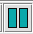
\includegraphics[width=0.5cm,height=0.5cm]{reflex_pause_button.png} - Pause the workflow execution.}
\item{
\includegraphics[width=0.5cm,height=0.5cm]{reflex_stop_button.png} - Stop the workflow execution.}
\end{itemize}
The remainder of the buttons (not shown here) are not relevant to the 
workflow execution.

%\subsubsection{Workflow States}
\subsection{Workflow States}

A workflow may only be in one of three states: executing, paused, or stopped.
 These states are indicated by the yellow highlighting of the

\includegraphics[width=0.5cm,height=0.5cm]{reflex_run_button.png},
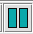
\includegraphics[width=0.5cm,height=0.5cm]{reflex_pause_button.png},
and 
\includegraphics[width=0.5cm,height=0.5cm]{reflex_stop_button.png}
buttons, respectively. A workflow is executed by clicking the

\includegraphics[width=0.5cm,height=0.5cm]{reflex_run_button.png} button. 
Subsequently the workflow and any running
pipeline recipe may be stopped immediately by clicking the

\includegraphics[width=0.5cm,height=0.5cm]{reflex_stop_button.png}
button, or the workflow may be paused by clicking the 
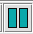
\includegraphics[width=0.5cm,height=0.5cm]{reflex_pause_button.png} button which
will allow the current actor/recipe to finish execution before the workflow is 
actually paused. 
After pausing, the workflow may be resumed by clicking the

\includegraphics[width=0.5cm,height=0.5cm]{reflex_run_button.png} button again.

